\chapter{Problem analysis}
\chlab{analysis}

In this chapter, we introduce the problems we aim to solve in this project. We start by providing a brief explanation of the chemical concepts behind molecule parameterisation~(\secref{chemical}). This is followed by the interaction design challenges for a fragment-based molecule parameterisation system in \secref{id_challenges}.



\section{Chemical concepts}
\seclab{chemical}
Every material is built up out of molecules, consisting of a set of atoms. Each of these atoms has a certain type, such as hydrogen~($H$) or carbon~($C$). The atoms of a molecule are connected via bonds, where there can be multiple bonds between the same atoms. Every atom is parameterised with a certain charge, which can be positive or negative, and is usually fractional. The molecule itself also has a charge, consisting of the sum of all its individual atom charges.

\begin{wrapfigure}{r}{.4\textwidth}
\vspace{-2em}
\begin{center}
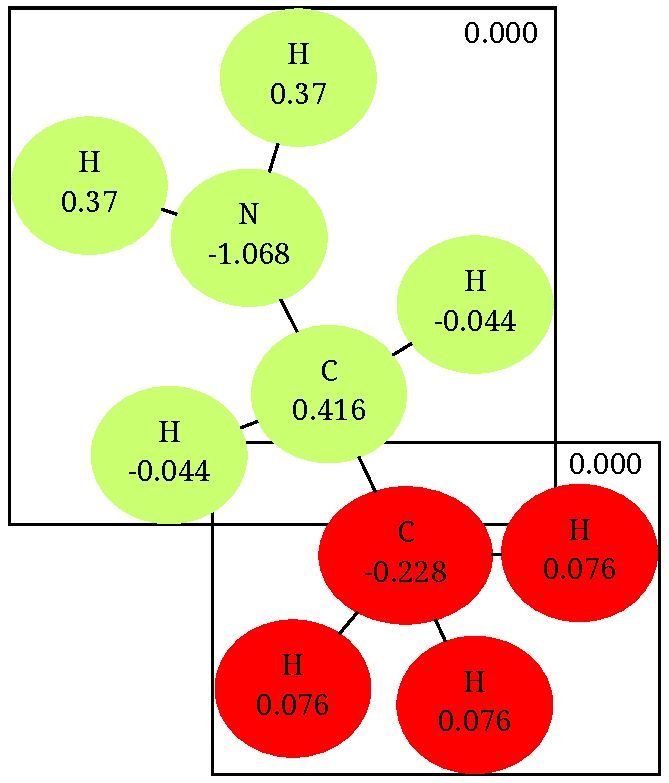
\includegraphics[width=.38\textwidth]{img/ethanamine.pdf}
\caption{Schematic view of ethanamine ($C_{2}H_{7}N$)~\cite{atb2014ethanamine}, including topology data on atom types, atomic charges and charge groups.}
\figlab{partial_charges}
\end{center}
\vspace{-2em}
\end{wrapfigure}

As mentioned in the introduction (\chref{introduction}), biomolecular simulations are becoming increasingly important, especially in the field of drug development. For these simulations, force field models are required to describe the interatomic relations of the drug molecules. In order to run a simulation, these force fields require the molecule's topology. This consists of the molecule's atom types, bonds, bond angles, atomic charges and charge groups.

\Figref{partial_charges} shows a schematic view of an ethanamine molecule. Here, every oval symbolises an atom, and the bonds are displayed as lines between the ovals. The atom type is the letter on the top rule of the oval, i.e.\ there are atoms of type $H$, $N$, and $C$ in the shown molecule. Atomic charges are given by the number at the bottom row~($-1.068$ for the $N$ atom). Finally, the colouring of the atoms and the boxes around them denote a charge group. This is a group of connected atoms, for which the total charge is ideally equal to that of the whole molecule ($0.0$ in this example).

In a recent study, El-Kebir, Klau et al. have developed an algorithm that allows for fast and reliable assignment of charge groups~\cite{canzar2012charge}. As this is now optimised, they currently focus on a different step in the parameterisation: that of calculating the atomic partial charges. Currently, these charges are retrieved using complex quantum-mechanical calculations. However, these calculations can take hours or even days to complete, and cannot be performed for larger molecules. As it is not believed that the algorithms used in these calculations can be improved much further, a different approach is needed for finding atom charges.

\begin{figure}[b!]
\centering
\makebox[\linewidth][c]{%
\begin{subfigure}[t]{0.5\textwidth}
\centering
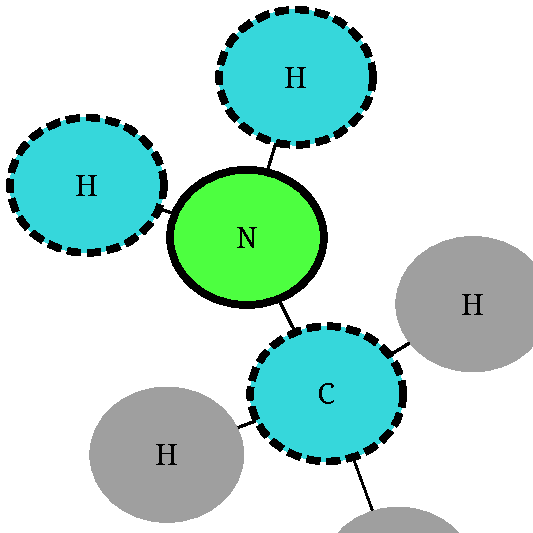
\includegraphics[width=.8\textwidth]{img/match_target.pdf}
\caption{Match target.}
\figlab{match_target}
\end{subfigure}%
\begin{subfigure}[t]{0.5\textwidth}
\centering
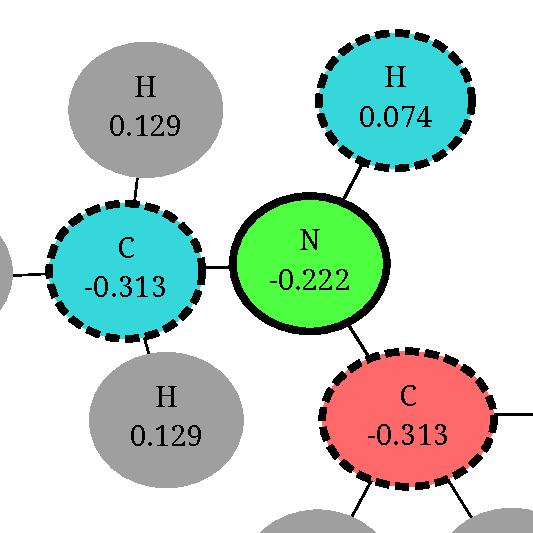
\includegraphics[width=.8\textwidth]{img/match_none.pdf}
\caption{Non-matching fragment.}
\figlab{match_none}
\end{subfigure}%
}\\[1em]
\makebox[\linewidth][c]{%
\begin{subfigure}[t]{0.5\textwidth}
\centering
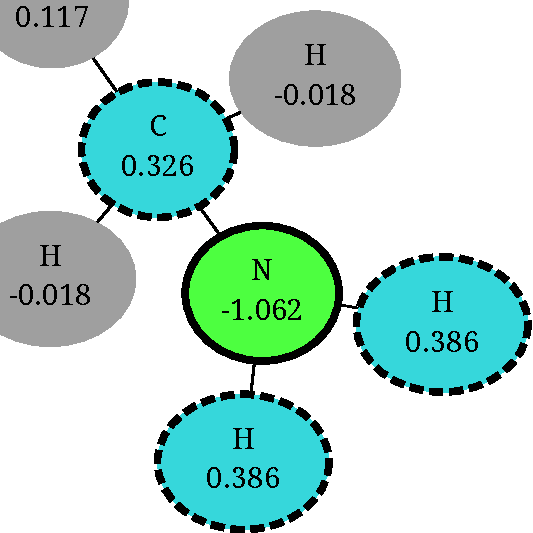
\includegraphics[width=.8\textwidth]{img/match_good.pdf}
\caption{Matching fragment.}
\figlab{match_good}
\end{subfigure}%
\begin{subfigure}[t]{0.5\textwidth}
\centering
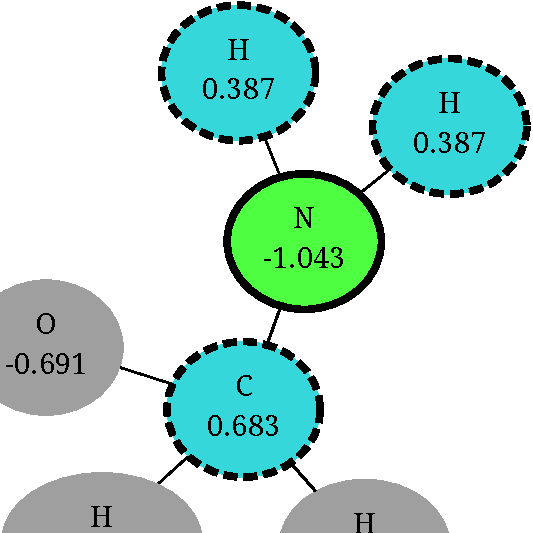
\includegraphics[width=.8\textwidth]{img/match_bad.pdf}
\caption{Matching fragment.}
\figlab{match_bad}
\end{subfigure}%
}
\caption{Basic fragment matching.}
\figlab{matching}
\end{figure}

A possible alternative method of finding atom charges is to exploit the similarity of molecules. The partial charges of an unparameterised molecule can be retrieved from similar fragments of other molecules for which the charges \emph{are} known. In \figref{matching}, the basics of fragment matching are shown. In this case, we are looking for an $N$ atom, with two connected $H$ atoms and a connected $C$ (see \figref{match_target}). As can clearly be seen, \figref{match_none} is not a match, as there are two $C$s connected to the $N$ atom there, and only one $H$. \Figref{match_good, match_bad} show two different fragments that \emph{do} match the target fragment. The $N$ atom is indeed connected to a $C$ and two $H$ atoms in both molecules. We will discuss fragment matching in more detail in \secref{impl_omfraf}.

As can be seen clearly for the $C$ atom in \figref{match_good, match_bad}, charges in similar fragments can still differ. This is due to the fact that atom charges are not only influenced by their direct neighbours, but also by the structure of the rest of the molecule. Due to this, it is not yet possible to fully automate the fragment-based molecule parameterisation process, as there are currently no known rules as to which aspects of the structure influence the charge in which way.

Instead of automating the process, a tool needs to be developed that allows experienced chemists to manually perform the parameterisation using fragments of other molecules. This tool should provide them with a list of matching fragments, and leave it to them to find the fragments that properly match with the molecule. In order to do this, users should be able to check all aspects of the found fragments, as these determine whether a fragment is a good match or not. Additionally, they need to be able to easily compare fragments, both with each other and with the target molecule.



\section{Research questions}
\seclab{id_questions}
From the short problem description provided in the previous section, we formulate the main research question for this project as follows:
\begin{quote}
How should chemists interact with a tool for fragment-based molecule parameterisation, such that using this tool yields results of comparable quality to using conventional methods, while taking less time to complete?
\end{quote}

This question can be split up into the following sub-questions:
\begin{enumerate}
\item Is it feasible to do manual partial charge assignment in a reasonable amount of time, i.e.\ faster than performing computations?
\item Compared to the computed charges, how accurate are the charges obtained using manual charge assignment?
\item How should chemists interact with a system for finding atomic partial charges using similar fragments of other molecules?
\end{enumerate}

The first of these sub-questions is potentially the most important one. When it would not be possible to complete a manual parameterisation in less time than performing computations, there would be no point in doing this manually. This would render the developed tool useless. Additionally, the obtained charges should also not deviate too much from the computed ones, as the results need to be accurate. Therefore, the answer to the second question can also make or break the tool. Finally, the answer to the third sub-question will influence the answers to the other ones, and finding it is the ultimate goal of this project.



\section[Challenges]{Interaction design challenges}
\seclab{id_challenges}
A system for fragment-based molecule parameterisation is not readily available. Therefore, a new system needs to be designed from the ground up. This allows for creating something completely new, but also creates the challenge of doing it right without having any clear starting point. In order to be able to validate the system, we implement two different versions of it and compare them.

Both implementations need to meet the same set of requirements. First of all, the system needs to provide its users with a view of the unparameterised molecule, and help them to find the best matching fragments. As the selected fragments may not always be perfect, it should also be possible for the users to manually adjust the charges for each atom, if they feel that this is needed.

In order to make sure users find the best available matching fragment, they should be encouraged to check as many fragments as possible. However, when many fragments are found, users should not have to compare all of them, as this might cost them way too much time. Therefore, the best matches should be easily recognisable, which requires the found fragments to be presented in a clear and intuitive way.

Another important requirement for the system is that is needs to support parameterisation of both small molecules, consisting of just a few atoms, and large molecules, being over a hundred atoms in size. This means that visualisation of the molecules should be given some thought, in order to make sure both large and small atoms are displayed correctly. It is particularly challenging to find a way to properly visualise large molecules on a screen with a limited size, so an approach is needed that allows for this.

Overall, the most important requirement for the system is to make it work intuitively and to implement it such that it makes chemists' work easier. Parameterising a large molecule should therefore not take hours to complete. Even if that would still be faster than calculating the charges, one can at least do something else while the computations are running. This, of course, is not possible while one has to focus on a manual parameterisation process.
